%\subsection{What has been accomplished?  What additional work needs to be done?}

\vspace{-2em}  % Reduce space after the figure
\section{Methodology}
\vspace{-2em}  % Reduce space after the figure

In the new iteration of HAM, numerous optimizations have been identified following nearly a decade of technological advancement. While improvements in circuitry and power delivery were a primary focus, several components from the original system had become outdated or obsolete, necessitating the selection and programming of modern replacements. To initiate the redesign process, students reviewed the original HAM project documentation, which outlined core components and movement logic. Gudi collaborated with members of the HAM (2015) team to draft an updated parts list, while Huong began analyzing the original mechanical systems and developing a comprehensive digital schematic for all pin connections. \par

\vspace{-2em}  % Reduce space after the figure
\section{Printed Circuit Boards}
\vspace{-2em}  % Reduce space after the figure

On the 2015 iteration of the project, HAM relied on a breadboard and jumper wires to connect all necessary components. While the system functioned as intended during flight, it posed challenges for post-flight maintenance and troubleshooting. In the 2025 iteration, HAM transitioned to using dedicated printed circuit boards (PCBs) for all subsystems. This shift improved modularity, simplified component replacement, and enabled systematic documentation for future development. \par

The system was divided into four PCBs, each serving a specific function: (1) the primary flight payload, (2) telemetry transmission, (3) video processing, and (4) mission control interface. Adopting PCBs not only streamlined the internal layout but also eliminated the bulk and complexity of breadboard wiring, resulting in a 10\% reduction in overall payload weight, as shown in Figure~\ref{Fig:Wiring_SideBySide}. \par

\begin{figure}[H]
    \centering
    \includegraphics[width=0.8\textwidth]{Figures/HAM_Wiring_Comparison.jpg}
    \caption{Side by side comparison of circuitry}
    \label{Fig:Wiring_SideBySide}
\end{figure}
\vspace{-2em}

These circuit boards incorporate design improvements that significantly enhance maintainability. Major upgrades include:

\vspace{-2em}
\begin{itemize}
    \item Dual power inputs (Anderson and 2.1~mm barrel jack) to accommodate both flight and ground configurations, replacing the previous setup of multiple Anderson connectors
    \item Integrated on/off power switch for streamlined testing and controlled power cycling
    \item Compact-form-factor ATmega2560 microcontroller for embedded control, replacing the larger Arduino Mega 2560 Rev 3
    \item Surface-mountable 1206 chip resistors, replacing legacy through-hole metal film resistors
    \item Modular hardware layout enabling easy component replacement and system reconfiguration
\end{itemize}

These improvements not only reduce the overall payload weight but also enhance the system’s reliability during both flight and testing. By transitioning to a more modular and compact design, the updated boards streamline troubleshooting and future development efforts. As a result, the HAM system is now better equipped to support extended missions and iterative upgrades across future launch campaigns.

\vspace{-2em}  % Reduce space after the figure
\section{Model Optimization}
\vspace{-2em}  % Reduce space after the figure

The original HAM model was 3D printed using PLA and designed to accommodate six servo motors. With a total weight of 15.4 ounces, the team identified the torso—accounting for 5 ounces—as a key target for weight reduction in future revisions. According to FAA guidelines, total payload stacks must not exceed a 12-pound weight limit~\cite{CFR_Part_101}; therefore, every ounce becomes critical at launch.

\begin{figure}[H]
    \centering
    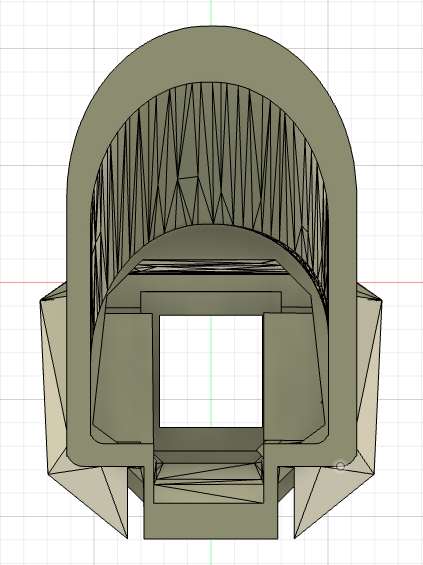
\includegraphics[width=0.24 \textwidth]{Figures/Model_Bottom_View.png}
    \caption{Bottom view of the updated Torso model}
    \label{Fig:Model_Bottom}
\end{figure}
\vspace{-2em}

The redesigned torso was split into two separate pieces to reduce the need for support material and improve print efficiency. This modular approach also simplifies maintenance, allowing for individual sections to be replaced without disassembling the entire body. Additionally, the internal structure was hollowed to minimize material usage, reducing the torso weight to 3.8 ounces. With all six servo motors installed, the complete model now weighs 11.9 ounces—an overall improvement of 22\% compared to the original design. \par

\vspace{-2em}  % Reduce space after the figure
\section{Additional Payloads}
\vspace{-2em}  % Reduce space after the figure

Alongside HAM’s telemetry and live-streaming systems, the overall flight stack will also include a dedicated communications payload to establish bidirectional data transfer between the flight system and the ground station. This will ensure reliable transmission of real-time telemetry during ascent and descent. Additionally,  we plan to integrate three supplementary payloads: (1) a 5.7k resolution 360° camera for flight documentation, (2) a SPOT Trace GPS tracker for redundancy in tracking and recovery, and (3) a venting system to regulate internal pressure and temperature of the balloon. These components were core elements of the University’s contributions to the Nationwide Eclipse Ballooning Project from 2022 to 2024 \cite{NEBP_Website}.